\documentclass[a4paper]{article}
\usepackage[spanish]{babel}
\usepackage[utf8]{inputenc}
\usepackage{fullpage} % Package to use full page
\usepackage{parskip} % Package to tweak paragraph skipping
\usepackage{tikz} % Package for drawing
\usepackage{amsmath}
\usepackage{amsfonts}
\usepackage{hyperref}
\usepackage{graphicx}
\usepackage{eucal}
\usepackage{algorithm}
\usepackage{algpseudocode}
\usepackage{float}
\usepackage{forest}
\usepackage{pgfplotstable}
\usepackage{pgfplots}
\usepackage[shortlabels]{enumitem}
\usepackage{caratula}

\algnewcommand{\IIf}[1]{\State\algorithmicif\ #1\ \algorithmicthen}
\algnewcommand{\EndIIf}{\unskip\ \algorithmicend\ \algorithmicif}
\algnewcommand{\LineComment}[1]{\State \(\triangleright\) #1}
\usepackage{mathtools}
\DeclarePairedDelimiter\ceil{\lceil}{\rceil}
\DeclarePairedDelimiter\floor{\lfloor}{\rfloor}

\usepackage{titlesec}

\setcounter{secnumdepth}{4}

\titleformat{\paragraph}
{\normalfont\normalsize\bfseries}{\theparagraph}{1em}{}
\titlespacing*{\paragraph}
{0pt}{3.25ex plus 1ex minus .2ex}{1.5ex plus .2ex}


\begin{document}
\newpage

\materia{Algoritmos y Estructuras de Datos III}
\submateria{Primer cuatrimestre 2017}
\titulo{TP Nº 2 - Grafos}
\subtitulo{Camino Minimo, Arboles} % opcional
\grupo{} % opcional
\integrante{Javier Petri}{306/15}{javierpetri2012@gmail.com}
\integrante{Jonathan Scherman}{152/15}{jonischerman@gmail.com}
\integrante{Lucas Adriel Figarola}{953/13}{lukas12\_alfa56@hotmail.com}
\integrante{Ruben Adrian Castiglione}{818/15}{adriancastiglione@gmail.com}

\maketitle
\thispagestyle{empty}
\newpage

\tableofcontents

%%\newpage
%%\section{Muestra}
%%
\section{Backtracking}
\begin{subsection}{Implementaci\'{o}n}

\begin{algorithm}[H]
  \begin{algorithmic}[1]
    \Function{BTPintar}{A, n, i, r, a}
      \If{i = 0} \Comment{Caso base} 
        \State \textbf{return} $0$
      \Else
      	\State ultimoElem $\gets$ A[i-1]
        \State minRamaR, minRamaA, minRamaSP$\gets$ n
		\If{$r = 0$ $\vee$ ultimoElem $<$ A[r-1]}
        	\State minRamaR $\gets$ BTPintar(A, n, i-1, i, a) \Comment{Pinto de rojo}
        \EndIf 
		\If{$a = 0$ $\vee$ ultimoElem $>$ A[a-1]}
        	\State minRamaA $\gets$ BTPintar(A, n, i-1, r, i) \Comment{Pinto de azul}
        \EndIf 
        \State minRamaSP $\gets$ BTPintar(A, n, i-1, r, a) + 1 \Comment{No lo pinto}
        \State \textbf{return} min(minRamaR, minRamaA, minRamaSP)
      \EndIf 
    \EndFunction
  \end{algorithmic}
\end{algorithm}

\end{subsection}

\vspace{1cm}
\pgfplotstableread[col sep=comma]{tiempos-bt.csv}{\table}
\begin{tikzpicture}
\begin{axis}[
  xlabel=Longitud ($n$),
  ylabel= $\log \text{Tiempo}(A)$ ($ms$),
  ymode = log ]
\addplot+[thin] table[x = length, y expr={\thisrow{ns_distribucion_uniforme}/1000}, col sep=comma]{\table};
\addlegendentry{A rnd.}
\addplot+[thin] table[x = length, y expr={\thisrow{ns_creciente}/1000}, col sep=comma]{\table};
\addlegendentry{A crec.}
\addplot+[thin] table[x = length, y expr={\thisrow{ns_decreciente}/(1000}, col sep=comma]{\table};
\addlegendentry{A decrec.}
\addplot+[thin] table[x = length, y expr={\thisrow{ns_constante}/1000}, col sep=comma]{\table};
\addlegendentry{A const.}
`\end{axis}
\end{tikzpicture}
\begin{tikzpicture}
\begin{axis}[
  xlabel=Longitud ($n$),
  ylabel= $\frac{\text{Tiempo}(A)}{3^n}$ ($ms$)
  ]
\addplot+[thin] table[x = length, y expr={\thisrow{ns_distribucion_uniforme}/(1000*3^\thisrow{length})}, col sep=comma]{\table};
\addlegendentry{A rnd.}
\addplot+[thin] table[x = length, y expr={\thisrow{ns_creciente}/(1000*3^\thisrow{length}}, col sep=comma]{\table};
\addlegendentry{A crec.}
\addplot+[thin] table[x = length, y expr={\thisrow{ns_decreciente}/(1000*3^\thisrow{length}}, col sep=comma]{\table};
\addlegendentry{A decrec.}
\addplot+[thin] table[x = length, y expr={\thisrow{ns_constante}/(1000*3^\thisrow{length}}, col sep=comma]{\table};
\addlegendentry{A const.}
`\end{axis}
\end{tikzpicture}

\newpage
\section{Delivery Optimo}


\begin{subsection}{Introducción al problema}

En este problema nos situaremos en una provincia de Optilandia, donde las ciudades están conectadas por rutas bidireccionales. Algunas de estas rutas (en general las que representan caminos más cortos y/o directos entre las ciudades) han sido catalogadas con la categoría de premium, indicando que se encuentran en mejor estado y que reciben mejor mantenimiento que el resto. Para reducir los costos del mismo existen regulaciones que impiden que una empresa de transportes utilice más de $k$ rutas premium en un mismo envío. Transportex es una de estas empresas y ha solicitado nuestros servicios para encontrar el camino de mínimo costo entre 2 ciudades (una de origen, otra de destino) cumpliendo con estas restricciones, siempre que esto sea posible.

Escribiremos un algoritmo que reciba los datos de las ciudades, las rutas y el $k$ permitido y encuentre una solución si es que existe. Las ciudades pueden interpretarse como los nodos de un grafo, y las rutas que las conectan como las aristas del mismo, por lo que interpretaremos la entrada como un grafo; también se sabe que siempre hay una forma de llegar de una ciudad a otra (independientemente del uso de rutas premium), por lo que este grafo será conexo. Llamaremos $n$ a la cantidad de nodos del grafo y $m$ al número de sus aristas. 

A partir del mismo construiremos un digrafo en el que los nodos serán tuplas  $\langle c, p \rangle$, representando que se puede llegar a la ciudad $c$ utilizando a lo sumo $p$ rutas premium. As\'{i}, 2 nodos estar\'{a}n conectados sii se puede pasar de un estado a otro, formalmente,  si $c_1$ y $c_2$ est\'{a}n conectadas en el grafo de entrada, $\langle c_1, p \rangle$ y $\langle c_2, p \rangle$ estar\'{a}n conectadas si las une una ruta normal, y $\langle c_1, p \rangle$ y $\langle c_2, p + 1\rangle$ estar\'{a}n conectadas si las une una ruta premium. 

Se construye un digrafo y no un grafo ya que si $c_1$ y $c_2$ est\'{a}n conectadas por una ruta premium, tiene sentido poder avanzar desde $\langle c_1, p \rangle$ hacia $\langle c_2, p+1 \rangle$ pero no al rev\'{e}s. Este digrafo tiene $n(k+1)$ nodos ya que se genera un nodo $\langle c_1, p \rangle$ para cada $c_1 \in [0; n)$ y para cada $p \in [0; k]$; en cuanto a las aristas, se generarán a lo sumo $k$ por cada arista incidente a $c_1$ en el grafo de entrada (este número cambiará en función de qué rutas sean premium y cuales no). En total, la cantidad de aristas del digrafo es, a lo sumo, $mk$.

Finalmente, obtendremos el camino m\'{i}nimo entre $\langle origen, 0 \rangle$ y $\langle destino, p \rangle$, $0 \leq p \leq k$, es decir, el camino m\'{i}nimo desde el origen, sin haber usado rutas premium (en realidad no se han usado rutas de ning\'{u}n tipo) y el destino, habiendo usado a lo sumo $p$ rutas premium. Es preciso notar que $k$ es el máximo número de rutas premium a utilizar, y que los caminos que utilicen menos también deben ser considerados, tomando de entre ellos el de mínimo costo.

\end{subsection}


\begin{subsection}{Representaci\'{o}n}
Representamos al grafo de entrada como una lista de adyacencia: para cada nodo se guardan sus vecinos junto con sus respectivas distancias.  Para simplicidad guardaremos la información sobre las rutas premium de la siguiente manera: si $d$ es la distancia (en valor absoluto) entre 2 ciudades, $d$ se guardará con signo negativo si esas ciudades est\'{a}n unidas por una ruta premium, y positivo cuando las une una ruta normal. Notar que $G$ es un grafo a pesar de esta representaci\'{o}n, y que la ciudad numerada como $i$ en el archivo de entrada será numerada como $i-1$ en la lista de adyacencia.
El nuevo digrafo se representa también con lista de adyacencia, donde cada vecino tiene el nodo correspondiente y la distancia. Dado que la información sobre si una ruta es premium o no está contenida en la conexión entre los nodos, las distancias se guardan positivas. Por lo tanto, un vecino es una tupla $\langle nodo, distancia \rangle$, donde los nodos son las tuplas $\langle c, p \rangle$ descriptas anteriormente y las distancias son números naturales.

\end{subsection}

\begin{subsection}{El algoritmo}
El algoritmo que resuelve el problema consta de 2 partes: la primera es la construcción del digrafo descr\'{i}pto anteriormente y la segunda la ejecución del algoritmo de Dijkstra sobre el mismo para encontrar los caminos minimos. Mostramos a continuación el armado del digrafo:

\begin{algorithm}[H]
  \begin{algorithmic}[1]
    \Function{Problema1-armarDigrafo}{grafoDeEntrada: listaAdyacencia$\langle int, int \rangle$ grafoEntrada, n: int, origen: int, destino: int, k}
    \State  grafo $\gets$ listaAdyacencia$\langle nodo, distancia \rangle$ de n(k+1) nodos
    \For{$i \in [0; n])$}
        \For{$v \in$ grafoDeEntrada.\textproc{vecinosDe($i$)}}
            \For{$p \in [0;k]$}
                \If{$p \neq k \wedge$ $i$ y $\Pi_1(v)$ están conectadas por una ruta premium}
                \State grafo.\textproc{AgregarVecino}($\langle i, p \rangle, \langle \langle \Pi_1(v), p+1 \rangle, |\Pi_2(v)|\rangle$)
                \ElsIf{$i$ y $\Pi_1(v)$ \underline{\textit{no}} están conectadas por una ruta premium}
                \State grafo.\textproc{AgregarVecino}($\langle i, p \rangle, \langle \langle \Pi_1(v), p \rangle, |\Pi_2(v)|\rangle$)
                \EndIf
            \EndFor
        \EndFor
    \EndFor
    
    \State \textbf{return} \textproc{caminoMinimoDijsktra}($\langle origen,0\rangle, \langle destino, k \rangle, grafo, k$)
    \EndFunction    
  \end{algorithmic}
\end{algorithm}

\end{subsection}

Como solo nos interesa la distancia desde el origen hacia un nodo en particular, sería interesante poder cortar la ejecución de Dijsktra una vez que esa distancia ha sido hallada. Recordemos brevemente el algoritmo:

\begin{algorithm}[H]
\begin{algorithmic}[1]

\Function{AlgoDijsktra}{Grafo G, nodo origen, nodo destino}

    \State Inicializar $\Pi$ distancias y $Q$ cola de prioridades
    \While{$Q$ no está vacia}
        \State $u \gets$ min($Q$)
        \For {each $v$ vertice vecino de $u$}
            \State procesar $v$
        \EndFor
    \EndWhile
    \State \textbf{return} $\Pi(destino)$
\EndFunction

\end{algorithmic}
\end{algorithm}

Este algoritmo mantiene un invariante en el \textbf{while}: en el momento en el que un vértice $u$ es extraido de la cola, se sabe que se ha obtenido su distancia mínima al origen. Aprovechando esta característica, nuestra implementación de Dijsktra deja de iterar cuando la cola no tiene más elementos, o cuando algún nodo $\langle destino, p \rangle$ ha sido extraido de la misma. Dado que $0 \leq p \leq k$ por como se construye el grafo, cualquier nodo sirve, ya que la cantidad exacta de rutas premium usadas no es importante. El algoritmo final es el siguiente:

\begin{algorithm}
\begin{algorithmic}[H]

\Function{AlgoDijsktra}{Grafo G, nodo origen, nodo destino}

    \State Inicializar $\Pi$ distancias y $Q$ cola de prioridades
    \While{$Q$ no está vacia}
        \State $u \gets$ min($Q$)        
        \If{NumeroNodo($u$) $=$ NumeroNodo(destino)}
            \State \textbf{return} $\Pi(u)$
        \EndIf
        

        \algstore{dijsktra-final}
        
\end{algorithmic}
\end{algorithm}

\begin{algorithm}
\begin{algorithmic}

        \algrestore{dijsktra-final}

        
        
        \For {each $v$ vertice vecino de $u$}
            \State procesar $v$
        \EndFor
    \EndWhile
    \State \textbf{return} $\Pi(destino)$
\EndFunction

\end{algorithmic}
\end{algorithm}


\begin{subsection}{Complejidad}

Llamemos $D=(V',X')$ al digrafo generado por el algoritmo, $n'=n(k+1)$ a la cantidad de sus nodos y $m'=m(k+1)$ al número de sus aristas. La complejidad de la solución estará dada por las complejidades de sus 2 partes.:
\begin{itemize}

\item La generación del del digrafo cuenta con 3 ciclos anidados. El exterior itera sobre todos los nodos, luego el siguiente ciclo itera sobre cada uno de sus vecinos. Esto da un total de $2m$ iteraciones entre ambos \textbf{for}s. El ciclo interior (que itera sobre $p$) realiza $(k+1)$ iteraciones (cada una de tiempo constante) por cada vecino del nodo $i$, es decir que el digrafo se construye en $2m(k+1)$ iteraciones, lo cual es O($mk$).
\item El algoritmo de Dijsktra se implementa utilizando una cola de prioridad con actualización de prioridades en O(1) e inicialización y búsqueda de mínimo en O($t$) (donde $t$ es la cantidad de elementos de la cola, la cuál se corresponde con $n'$). Se harán $n'$ extracciones de mínimo y $m'$ actualizaciones de prioridades, obteniéndose una complejidad de O($(n')^2 + m'$), o lo que es lo mismo, O($(nk)^2 + mk$). 
\end{itemize}

Juntándose ambas las partes, el algoritmo correrá en O($(nk)^2 + mk$). Sabiendo que $m \leq n^2$, se puede afirmar que O($mk$) $\in$ O($n^2k$) $\in$ O($(nk)^2$).

\subsection{Correctitud}

Nuestra solución interpreta el mapa de entrada como un grafo $G=(V,X)$ y arma un digrafo $D=(X',V')$ para luego ejecutar el algoritmo de Dijskstra sobre él. Dado que éste algoritmo es correcto, bastará con demostrar que $D$ sirve efectivamente para resolver el problema. Llamemos $G_k$ al grafo (mapa) de entrada, restringido a los caminos que tienen hasta $k$ rutas premium, y $G - G_k$ al grafo (mapa) de entrada restringido a rutas de más de $k$ rutas premium. Demostrar que $D$ sirve para nuestro problema es equivalente a demostrar las siguientes 4 propiedades:


\begin{enumerate}
\item Todos los caminos de $G_k$ están en $D$
\item Todos caminos de $G - G_k$ no están en $D$
\item Para todo camino de hasta $k$ rutas premium, su costo en $G_k$ es el mismo que en $D$
\item Todos los caminos de $D$ están en $G_k$
\end{enumerate}

Si éstas propiedades son ciertas, buscar un camino mínimo en $G_k$ es equivalente a buscar un camino mínimo en $D$. 

Comencemos con algunas definiciones:
\begin{itemize}
\item Llamaremos $x_{ij} \in X$ a la arista que conecta los vértices $v_i$ y $v_j$ en $G$. 

\item Llamaremos $w(x)$ a la función de costo de las aristas de $G$ y $w'(x)$ a la función de costo de las aristas de $D$.

\item $(v_i, p) \in V'$, $\forall v_i \in V, \forall p \leq k$

\item Si $x_{ij}$ es una ruta premium, $\langle v_i, p \rangle$ estará conectada con $\langle v_j, p+1 \rangle$ en $D$ tal que $w(x_{ij}) = w'((\langle v_i, p\rangle, \langle v_j, p+1\rangle))$ (donde $p$ es la cantidad de rutas premium usadas hasta $v_i$ en el camino del que $v_i$ y $v_j$ son parte).

\item Si $x_{ij}$ es una ruta no premium, $\langle v_i, p \rangle$ estará conectada con $\langle v_j, p \rangle$ en $D$ tal que $w(x_{ij}) = w'((\langle v_i, p\rangle, \langle v_j, p\rangle))$ (donde $p$ es la cantidad de rutas premium usadas hasta $v_i$ en el camino del que $v_i$ y $v_j$ son parte).

\end{itemize}

Ahora sí, demostremos una a una las propiedades.

\subsubsection*{Los caminos de $G_k$ están en $D$.}

Sea $v_1, ..., v_n$ un camino $v_1$ hasta $v_n$ con $\lambda$ rutas premium, $v_i \in V$, $\lambda \leq k$. Notemos que este es un camino entre 2 nodos cualesquiera y que el nombre de los nodos es meramente orientativo, es decir, $n$ es la longitud del camino y $v_i$ es el $i$-ésimo nodo del mismo. Sea $P_1(n) = \exists (v_1, 0), ..., (v_n, \lambda )$ en $D$. Demostremos $(\forall n_0 \leq n)(P_1(n_0))$ por inducción en la longitud del camino.

\textbf{C.B.}: 
$P_1(1)$  es cierto pues $v_1$ es un camino de un único nodo, sin aristas, y se corresponde con el camino $(v_1, 0)$ en $D$.

\textbf{H.I.}: $P_1(t)$ es cierto $\forall t \leq n-1$

\textbf{T.I.}: 
\begin{itemize}

\item Si $x_{(n-1)n}$ es una ruta premium entonces el camino $v_1, ..., v_{n-1}$ utiliza $\lambda -1$ rutas premium. Por H.I. existe un camino de $(v_1, 0)$ a $(v_{n-1}, \lambda-1)$. Según las reglas de construcción del digrafo este nodo se conecta con $(v_{n}, (\lambda -1) + 1) = (v_{n}, \lambda)$. Entonces existe un camino de $(v_1, 0)$ a $(v_n, \lambda)$.

\item $x_{(n-1)n}$ es una ruta \textit{no} premium entonces el camino $v_1, ..., v_{n-1}$ utiliza $\lambda$ rutas premium. Por H.I. existe un camino de $(v_1, 0)$ a $(v_{n-1}, \lambda)$. Según las reglas de construcción del digrafo este nodo se conecta con $(v_{n}, \lambda)$. Entonces existe un camino de $(v_1, 0)$ a $(v_n, \lambda)$.

\end{itemize}

\subsection*{Todos caminos de $G - G_k$ no están en $D$}

Sea $v_1, ..., v_n$ un camino de $v_1$ hasta $v_n$ con $\lambda$ rutas premium, $v_i \in V$, $ k < \lambda$. Nuevamente, $n$ es la longitud del camino y $v_i$ su $i$-ésimo nodo. Sea $v_t$ un nodo de este camino, $t < n$, tal que $v_1, ..., v_t$ utiliza $k$ rutas premium y tal que $x_{t(t+1)}$ es una ruta premium. Este nodo existe porque el camino completo utiliza al menos $k+1$ rutas premium. Por $P_1(t)$ existe un camino $(v_1, 0)$ a $(v_t, k)$ en $D$. Según las reglas de construcción del digrafo, $(v_t, k)$ debe conectarse con $(v_{t+1}, k+1)$, pero este último nodo no pertenece a $D$ por definición, entonces el camino completo \textit{no} pertenece a $D$.

\subsection*{Para todo camino de hasta $k$ rutas premium, su costo en $G_k$ es el mismo que en $D$}

Sea $v_1, ..., v_n$ un camino de $v_1$ hasta $v_n$ con $\lambda$ rutas premium, $v_i \in V$, $ k < \lambda$, $n$ longitud del camino y $v_i$ su $i$-ésimo nodo. Sea $C_n = \sum_{i = 1}^{i \leq n-1} w(x_{i(i+1)})$ el costo total de este camino. Por $P_1(n)$ existe un camino $v_1' = (v_1, 0), ..., v_n' = (v_n, \lambda)$; sea $C_n' = \sum_{i = 1}^{i \leq n-1} w'((v_i', v_{i+1}'))$ el costo de este camino. Sea $P_2(n) = (C_n = C_n')$. Demostraremos $(\forall n_0 \leq n)(P_2(n_0))$ por inducción en $n$:

\textbf{C.B.}: 
$v_1$ es un camino de costo cero, pues no tiene aristas. $v_1'=(v_1, 0)$ es un camino de un único nodo que tampoco usa aristas y por tanto su costo también es cero. Luego $P_2(1)$ es verdadero. 

\textbf{H.I.}: $P_2(t)$ es cierto $\forall t \leq (n-1)$

\textbf{T.I.}: 
Por $P_1(n)$, $v_n' = (v_n, \lambda)$ es el último nodo del camino correspondiente en $D$. Por reglas de construcción del digrafo, el nodo anterior a éste es $v_{n-1}' = (v_{n-1}, p)$, con $p \in \{ \lambda, \lambda - 1 \}$, y se conecta con $(v_n, \lambda)$ mediante una arista de mismo costo que $x_{(n-1)n}$.

Por definición, $C_n = C_{n-1} + w(x_{(n-1)n})$ y $C_n' = C_{n-1}' + w'((v_{n-1}', v_n'))$. Por reglas de construción del digrafo, $w(x_{(n-1)n}) = w'((v_{n-1}', v_n'))$ y por H.I. $C_{n-1} = C_{n-1}'$, entonces $C_n = C_n'$.


\subsection*{Todos los caminos de $D$ están en $G_k$}

Sea $v_1', ..., v_n'$ un camino en $D$ tal que $v_n' = (v_n, \lambda)$, con $n$ la longitud del grafo y $v_i$ el $i$-ésimo nodo del camino. Sea $P_3(n) = \exists v_1, ..., v_n$ camino en $G$ de $\lambda$ rutas premium. Demostraremos $(\forall t \leq n)P_3(t)$ por inducción en la longitud del camino.  Como por definición $\lambda \leq k$, si $P_3(n)$ es verdadera entonces el camino estará en $G_k$.

\textbf{C.B.}: $v_1'$ es un camino de un único nodo que no usa ningún tipo de rutas, por lo tanto $\lambda = 0$ y $v_1' = (v_1, 0)$. Como $v_1 \in V$, $v_1$ es un camino de un único nodo en $G$ que usa 0 rutas premium. Por lo tanto $P_3(1)$ es verdadera. 

\textbf{H.I.}: $P_3(t)$ es cierto $\forall t \leq n-1$

\textbf{T.I.}: $v_n' = (v_n, \lambda)$ es el último nodo del camino. Por reglas de construcción del digrafo, el nodo anterior a este es o bien $(v_{n-1}, \lambda - 1)$ (y $x_{(n-1)n}$ es una ruta premium), o bien $(v_{n-1}, \lambda)$ (y $x_{(n-1)n}$ es una ruta no premium).

\begin{itemize}

\item Si el nodo anterior es $(v_{n-1}, \lambda - 1)$: Por H.I. existe $v_1, ..., v_{n-1}$ camino en $G$ con $\lambda - 1$ rutas premium. Como $x_{(n-1)n}$ es una ruta premium, el camino $v_1, ..., v_{n-1}, v_n$ utiliza $\lambda$ rutas premium.

\item Si el nodo anterior es $(v_{n-1}, \lambda)$: Por H.I. existe $v_1, ..., v_{n-1}$ camino en $G$ con $\lambda$ rutas premium. Como $x_{(n-1)n}$ es una ruta no premium, el camino $v_1, ..., v_{n-1}, v_n$ también utiliza $\lambda$ rutas premium.

\end{itemize}

Todas las propiedades son válidas, por lo tanto buscar el camino mínimo entre 2 nodos en $G_k$ es equivalente a buscarlo en $D$ y por tanto el digrafo no altera las soluciones. Luego el algoritmo es correcto. 

\subsection{Experimentaci\'{o}n}

Para la experimentaci\'{o}n realizamos un generador de instancias aleatorias para este problema, que genera grafos de $n$ nodos, $m$ aristas (de las cuales $p$ son premium) y busca un camino m\'{i}nimo de $origen$ a $destino$ usando $k$ rutas premium ($n, m, p, origen, destino, k$ son par\'{a}metros para el generador) . El algoritmo del generador puede ser simplificado en 3 pasos:
\begin{itemize}
    \item Generar un camino de $n$ nodos de manera aleatoria
    \item Generar aristas entre nodos aleatorios (siempre y cuando no estuvieran conectados previamente ni sean el mismo nodo) hasta completar a $m$ ($m$ se establece entre $n-1$ y $\frac{n(n-1)}{2}$).
    \item Seleccionar $p$ aristas aleatoriamente y catalogarlas como rutas premium.
\end{itemize}

Para generar el camino se selecciona un nodo aleatoriamente como inicial, y se lo marca como el nodo actual. Luego, sobre los nodos que no han sido seleccionados se selecciona un nuevo nodo aleatoriamente, se lo convierte en vecino del nodo actual y se lo marca como el nuevo nodo actual. Este proceso se repite hasta que no queden nodos que no hayan sido seleccionados. Para el segundo y tercer paso simplemente se seleccionan nodos aleatorios y se los une o marca su ruta como premium si las condiciones están dadas; en ambos casos se descartan aquellos nodos seleccionados y que no cumplan las condiciones para asegurar que el algoritmo termine. En cuanto a las condiciones, se unen nodos distintos que no hayan sido unidos previamente y se marca como premium el camino entre dos nodos sii estos están unidos y su ruta no es premium.
Para la selecci\'{o}n aleatoria se utiliza la funci\'{o}n \textproc{rand} de C++.

A continuación se harán experimentaciones para medir complejidades y para analizar casos buenos y malos para esta solución (en términos de complejidad).

\subsubsection{Mediciones de complejidad}

El objetivo de esta experimetaci\'{o}n es el de comprobar que las complejidades te\'{o}ricas se cumplan en la implementaci\'{o}n. Dado que la misma depende de las variables $n$, $k$ y $m$, se realizarán experimentaciones para medir cada una de ellas por separado, fijando las otras 2. Recordemos que la complejidad teórica analizada es de O($n^2k^2 + mk$), con $mk \in$ O($n^2k^2$).

\paragraph{Complejidad sobre $n$}

Para este primer experimento $k$ y $m'$ serán fijadas en 2000 y 20 respectivamente, mientras que $n$ aumentará de 100 hasta 500 dando saltos de a 10. Dicho de otro modo, se probarán instancias de tamaño $n = 100, 110, 120, ..., 500$, midiendo sus tiempos de ejecución. Para cada caso se harán 5 repeticiones y se tomará la mediana. Se espera que el crecimiento sea cuadrático, por lo que una vez obtenidos los resultados se calculará el coeficiente de pearson junto con las funciones $n$, $n^2$, $n^3$ y $n^4$ para medir la correlación de estas con los tiempos de corrida. Dado que todos son polinomios la correlación debería ser alta en todos los casos, pero $n^2$ debería tener la mayor correlación de acuerdo al análisis teórico. A continuación los resultados:

\hspace*{-1cm}{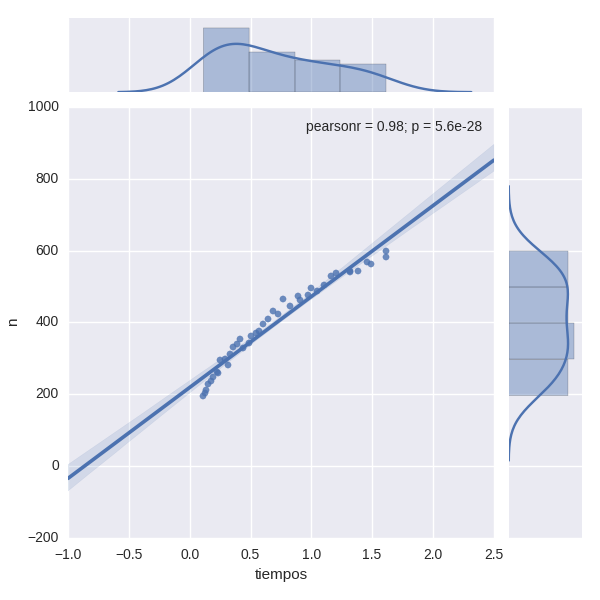
\includegraphics[width=8cm,height=8cm,keepaspectratio]{img/testn_n.png}}
\hspace*{-1cm}{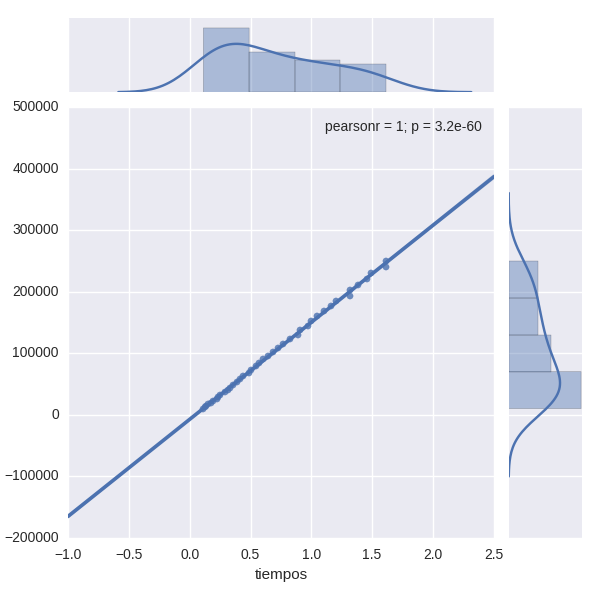
\includegraphics[width=8cm,height=8cm,keepaspectratio]{img/testn_n2.png}}

\hspace*{-1cm}{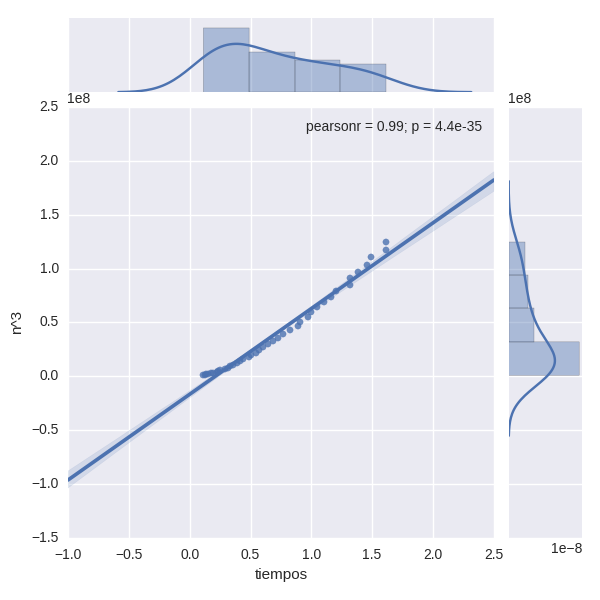
\includegraphics[width=8cm,height=8cm,keepaspectratio]{img/testn_n3.png}}
\hspace*{-1cm}{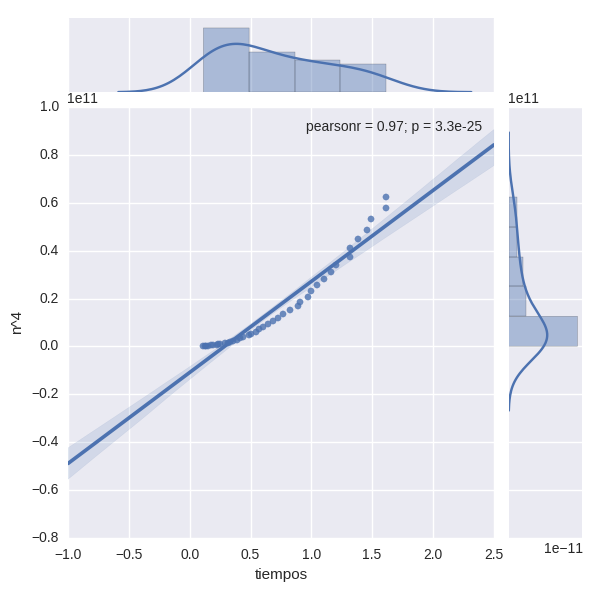
\includegraphics[width=8cm,height=8cm,keepaspectratio]{img/testn_n4.png}}

Tal como se esperaba, los coeficientes son altos en todos los casos, sin embargo la correlación entre los tiempos de corrida del algoritmo y la función $n^2$ es perfecta, por lo tanto el crecimiento de $n$ es cuadrático, tal como surgió del análisis teórico. Observar que la correlación con $n^3$ es casi perfecta (sin embargo con una probabilidad de error ligeramente mayor), lo cual sugiere que la constante que acompaña a la complejidad de la solución es grande en comparación con los tamaños de muestra y que con $n$ de mayor tamaño la diferencia será más notoria. 

\paragraph{Complejidad sobre $k$}

En este caso se fijarán $n$ y $m$ en 100 y 2000 mientras que $k$ aumentará desde 100 hasta 500 dando saltos de a 10. Nuevamente se miden tiempos de ejecución, se realizan 5 repeticiones para caso (tomando la mediana de las 5), y se mide la correlación con $n$, $n^2$, $n^3$ y $n^4$ mediante el coeficiente de pearson. También en este caso se espera que el crecimiento sea cuadrático. 

\hspace*{-1cm}{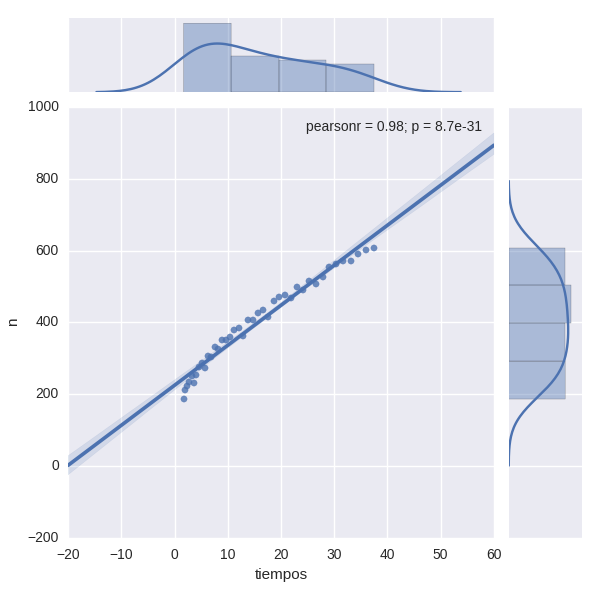
\includegraphics[width=8cm,height=8cm,keepaspectratio]{img/testk_n.png}}
\hspace*{-1cm}{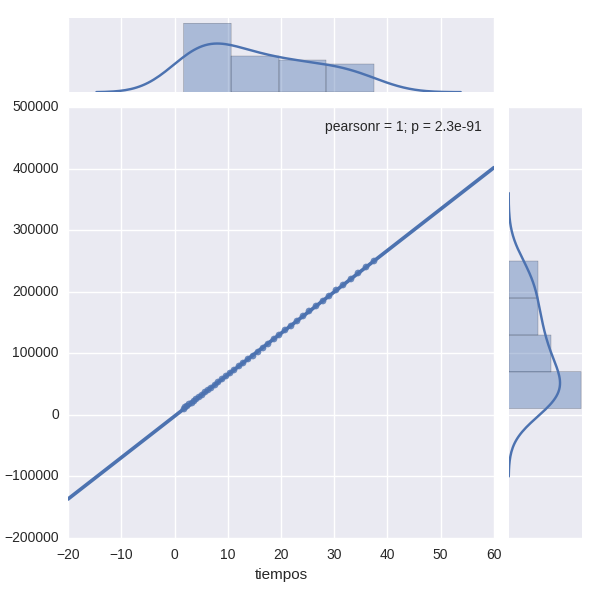
\includegraphics[width=8cm,height=8cm,keepaspectratio]{img/testk_n2.png}}

\hspace*{-1cm}{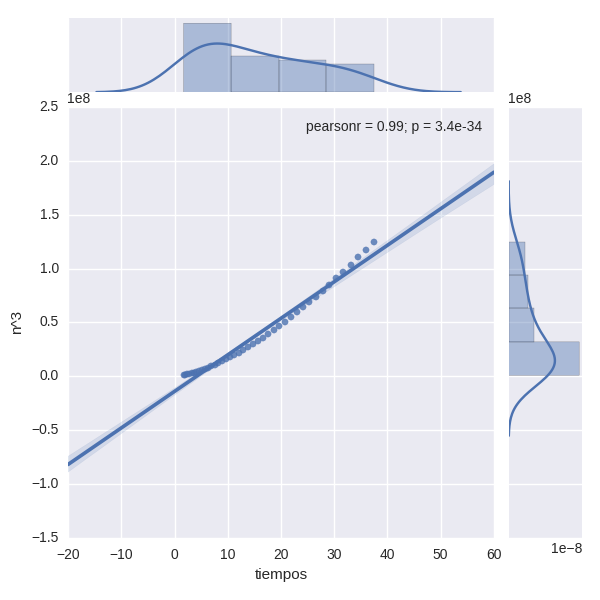
\includegraphics[width=8cm,height=8cm,keepaspectratio]{img/testk_n3.png}}
\hspace*{-1cm}{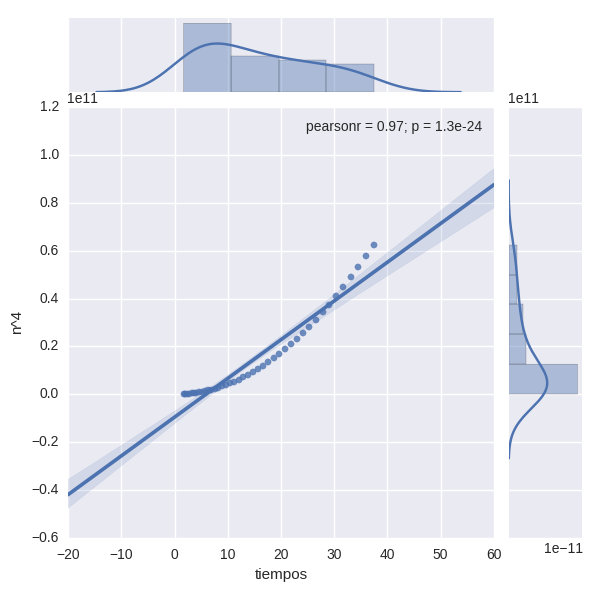
\includegraphics[width=8cm,height=8cm,keepaspectratio]{img/testk_n4.png}}

Nuevamente la correlación entre los tiempos obtenidos y $n^2$ es perfecta, indicando que el crecimiento de la función es cuadrático en $k$. Nuevamente la correlación con $n^3$ es casi perfecta (y con mayor margen de error), sugiriendo, al igual que $n$, la diferencia será más notoria con muestras mayores debido a las constantes que acompañan a las funciones de complejidad. 


\paragraph{Complejidad sobre $m'$}

Se fijarán $n$ y $k$ en 1000 y 20 y $m'$ se moverá entre 1000 y 4950 dando saltos de a 50. Nuevamente se realizarán 5 repeticiones y se tomará la mediana de los tiempos obtenidos. En cuanto al resultado esperado, se espera que el crecimiento sea lineal con respecto a $n$, por lo que en este caso los tiempos de corrida se correlacionarán con la función constante y con las funciones $n$, $n^2$ y $n^3$. A continuación presentamos los resultados:

\hspace*{-1cm}{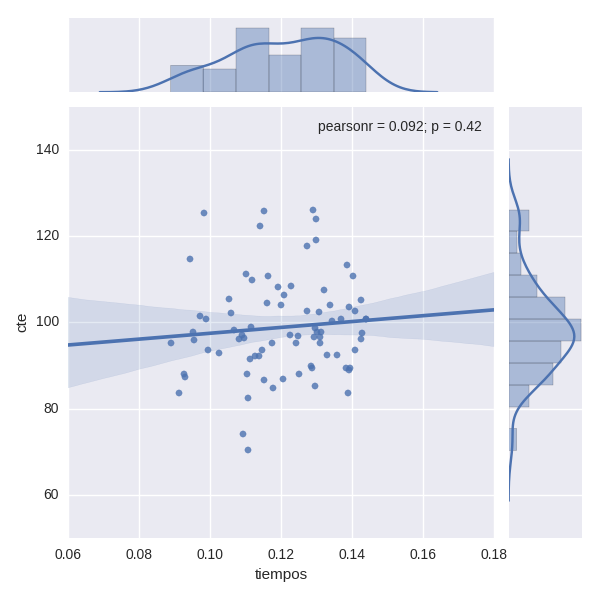
\includegraphics[width=8cm,height=8cm,keepaspectratio]{img/testm_cte.png}}
\hspace*{-1cm}{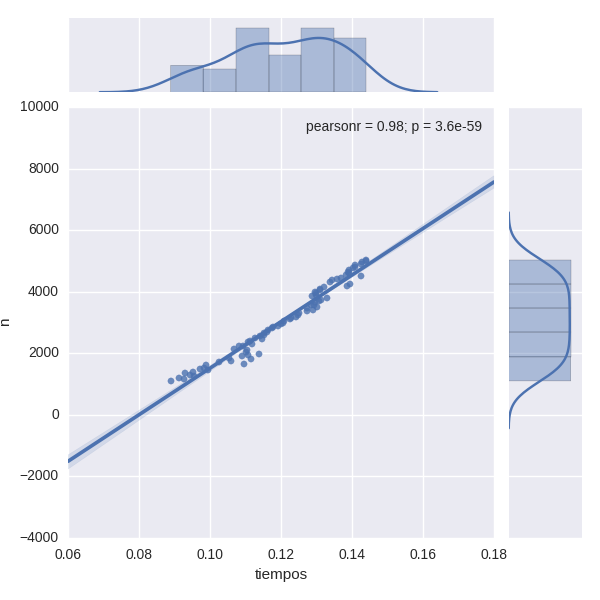
\includegraphics[width=8cm,height=8cm,keepaspectratio]{img/testm_n.png}}

\hspace*{-1cm}{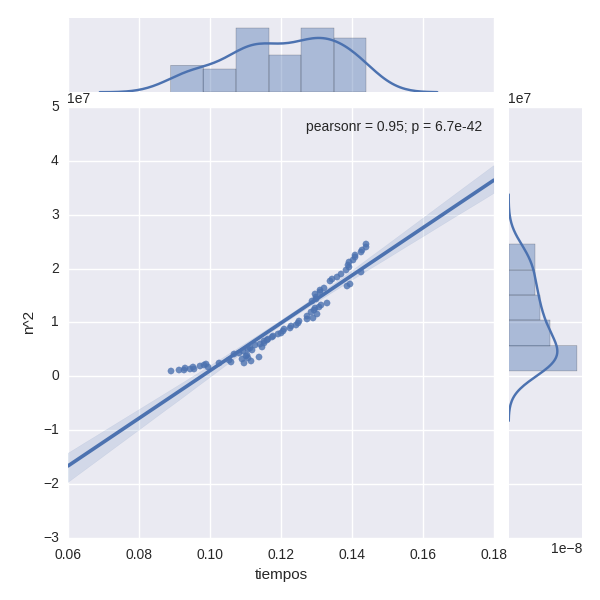
\includegraphics[width=8cm,height=8cm,keepaspectratio]{img/testm_n2.png}}
\hspace*{-1cm}{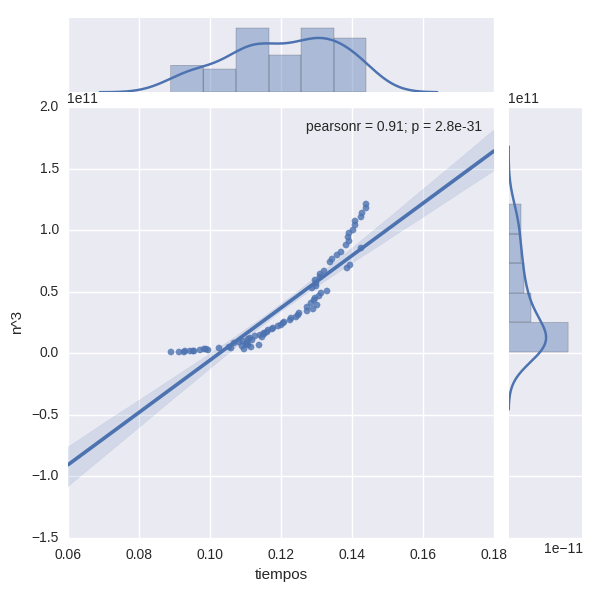
\includegraphics[width=8cm,height=8cm,keepaspectratio]{img/testm_n3.png}}

Si bien ninguna de las funciones expuestas se correlaciona perfectamente con los tiempos obtenidos (cosa que \textit{si} pasaba en los casos anteriores, la función lineal es la que mejor correlación, sugiriendo que afirmar que el crecimiento es lineal con respecto a $m$ es lo más cercano a la realidad. Notar que como $m \in $ O($n^2k^2$), podría usarse esta última cota de complejidad para toda la solución, lo cual sugeriría que el crecimiento en $m$ tendría que ser constante. Sin embargo, observar que la función constante esta muy poco correlacionada con los tiempos obtenidos, por lo que utilizar esta cota sería perder información sobre los tiempos reales del algoritmo. 


\subsubsection{Casos buenos y malos}

En nuestra implementación del algoritmo de Dijkstra agregamos un corte para que, una vez que un nodo que contenga la ciudad de destino sea desencolado, el algoritmo pare y devuelva la distancia hallada. Mediremos esta condición de corte con un gráfo de ?? nodos que consistirá en un único camino. Así, si $G=(V,X)$ es el éste grafo, $V=\{n: 1 \leq n \leq 5000\}$ y $X=\{ (i, i+1) : 0 \leq i \leq 5999 \}$. Fijaremos $k$ en 2, sin embargo ninguna ruta será premium. Así, $n$, $m$ y $k$ quedan fijados en 5000, 4999 y 2 respectivamente. Estableceremos al nodo 1 como origen e iremos moviendo el nodo de destino desde 1000 hasta 5000 aumentando de a 100. Mediremos los tiempos de corrida, corriendo cada caso 5 veces y tomando la mediana:

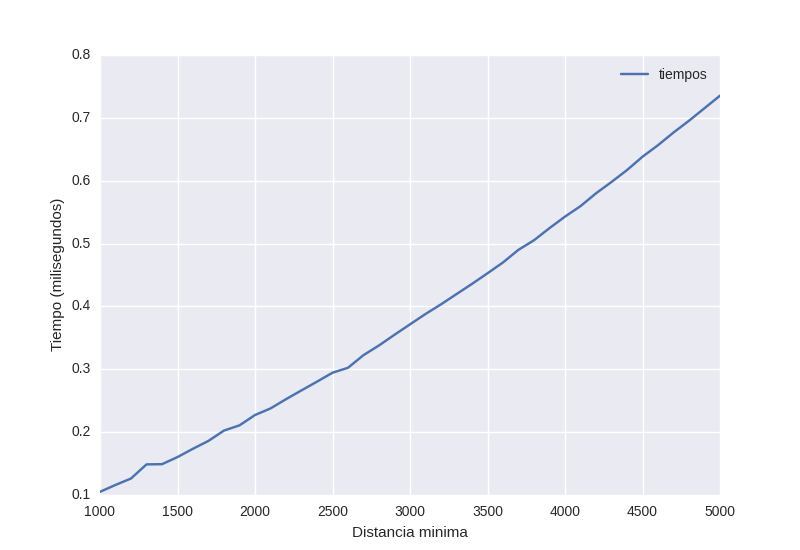
\includegraphics[width=15cm,height=15cm,keepaspectratio]{img/caso_dist.png}

La variación de tiempos es lineal porque en los casos de test el destino cambia (crece) de forma lineal. Lo importante en este caso no es el tipo de crecimiento sino que efectivamente se observan cambios en los tiempos de corrida del algoritmo. Esto quiere decir que, gracias a la condición de corte extra en el algoritmo de Dijkstra, el tiempo total que tarda en correr el algoritmo se reduce según el camino mínimo que se esté buscando. Dicho de otra forma, si el nodo de destino es encontrado rápidamente, solo estaremos obligados a pagar el costo de armar el digrafo, sumado a las iteraciones que haga Dijkstra. Si bien esto no cambia las complejidades teóricas, sí podemos afirmar que en la práctica pueden lograrse tiempos mejores que los analizados. 






\end{subsection}



\newpage
\section{Subsidiando el transporte}

\begin{subsection}{Representaci\'{o}n}
Representaremos este problema con un grafo $G$ que cumpla lo siguiente:
\begin{itemize}
	\item{$G$ es un grafo orientado: Nos dicen que las rutas son de mano \'{u}nica por lo que representaremos estas rutas como aristas orientadas.}
    \item{$V = \{v \in \mathbb{N}_0 : v < n \}$: Esto es, los v\'{e}rtices de $G$ ser\'{a}n n\'{u}meros, en donde cada uno de ellos representa cada una de las $n$ ciudades del problema.}
    \item{$E = \{(v_1, v_2) \in V^2 : \text{$\exists$ ruta que va de $v_1$ a $v_2$}  \}$: De esta forma, los ejes de $G$ representar\'{a}n las rutas del problema.}
    \item{$p:E \rightarrow \mathbb{Z}$: Representaremos los precios de los peajes como pesos en los ejes (si son positivos, ser\'{a}n la suma que se cobra al cliente. Si son negativos, la suma que se le paga). Para ello, la funci\'{o}n $p$ asignar\'{a} enteros a cada uno de estos. Notar que nos dicen que hay un peaje por cada ruta por lo que $dom(p)=E$ ya que cada peaje debe tener un costo.  }
    \item{$\forall v \in V, {d_{out}}(v) \geq 1$ (no existen ciudades aisladas)}

\end{itemize}
Entonces, $G$ ser\'{a} el modelo que representa a la ciudad de nuestro problema. Puntualmente, lo que queremos es encontrar el m\'{a}ximo $s$ tq si consideramos $p'(e) = p(e) - s$ $(\forall e \in E)$ en lugar de $p$, entonces no se forman ciclos negativos, es decir, que la suma de los pesos de sus ejes no sea menor a 0. \\ \\ 
Para constru\'{i}r $G$ a partir de la entrada, lo que haremos ser\'{a} ir agregando eje por eje, que va a tomar $O(m)$. Representaremos as\'{i} a $G$ como una lista de incidencias.
\end{subsection}


\begin{subsection}{Resoluci\'{o}n}
La idea para la resoluci\'{o}n del problema va a ser la siguiente:
\begin{enumerate}
	\item{Unir un v\'{e}rtice \textit{centinela} a cada uno de los nodos: En el siguiente punto vamos a necesitar usar el algoritmo de \textit{Bellman-Ford} en $G$. Como no sabemos si $G$ es fuertemente conexo o no,  agregamos este centinela que alcance a todos los $v \in V$, para luego correr el algoritmo tomando al centinela como origen.}
    \item{Variar subsidio $0 \leq s \leq C$ binariamente hasta encontrar el m\'{a}ximo:  
    \begin{itemize}
    	\item{Se va a ir probando con subsidios que van a variar como en una b\'{u}squeda binaria tradicional. La diferencia es que, en cada iteraci\'{o}n, se va a fijar si tal subsidio genera alg\'{u}n ciclo negativo en lugar de verificar si el elemento actual es el buscado.}
    	\item{Para encontrar ciclos negativos, se utiliza el algoritmo de \textit{Bellman-Ford}, tomando como origen al centinela agregado en el paso 1 que, como alcanza a todos los v\'{e}rtices de $G$, nos asegura que encuentra todos los ciclos negativos en caso que los hubiera.}
        \end{itemize}
        }
\end{enumerate}
De esta forma, una vez que tengamos maximizado el s del paso 2, sabremos que ese es el valor m\'{a}ximo para el cual no se generan ciclos negativos que, en terminos del problema, corresponde al m\'{a}ximo subsidio que se puede aplicar tal que no genere aprovechamientos, lo cual es la soluci\'{o}n \'{o}ptima al problema que pretendemos resolver.  
\end{subsection}

\begin{subsection}{Implementaci\'{o}n}
Para la implementaci\'{o}n del algoritmo, vamos a usar la funci\'{o}n \textit{hayCicloNegativo?} que, mediante el algoritmo de \textit{Bellman-Ford}, detecta si hay ciclos negativos en el grafo. Para ello, le pasamos como par\'{a}metro el grafo con sus dimensiones y el nodo origen, que  en este caso ser\'{a} el centinela puesto que es el \'{u}nico v\'{e}rtice para el cual podemos asegurar que est\'{a} conectado a todos los nodos del grafo y as\'{i} no se va a perder ning\'{u}n ciclo negativo en caso que los haya. \\
Adem\'{a}s, usaremos las funci\'{o}n \textit{aumentarSubsidio} que recibe las rutas y una constante por par\'{a}metro y, entonces,  para cada ruta, le resta la constante a su peso. De forma similar tendremos la funci\'{o}n \textit{disminu\'{i}rSubsidio} que, en lugar de restar la constante para cada ruta, la suma. 
\begin{algorithm}[H]
  \begin{algorithmic}[1]
    \Function{maximoSubsidio}{rutas, n, m, C}
    \State centinela $\gets$ n
    \For{i=1 to n} \Comment{Unir centinela a todos los nodos}
    	\State e $\gets$ Eje(centinela, n, C)
    	\State rutas.push(e)
        \State m++
    \EndFor
    \State n++
	\State j $\leftarrow$ C
    \State i $\leftarrow$ 0
    \State s, sAnterior $\leftarrow$ 0
    \While{i $<$ j}\Comment{Mover binariamente $s$}
    \State s $\leftarrow \floor{\frac{j+i}{2}}$ 
    \IIf{s = sAnterior} \textbf{return} s \EndIIf \Comment{Evita ciclo infinito en caso borde}
    \State aumentarSubsidio(rutas, s)
     \If{hayCicloNegativo?(rutas, n, m, centinela)}
     \State{j $\leftarrow$ s}
     \Else
     \State i $\leftarrow$ s
     \EndIf
    \State disminu\'{i}rSubsidio(rutas, s)
    \State sAnterior = s
    \EndWhile
    \State \textbf{return} s
    \EndFunction    
  \end{algorithmic}
\end{algorithm}
\end{subsection}


\begin{subsection}{Complejidad}
En el primer ciclo (L3-7) se ejecuta n veces operaciones que son $O(1)$ por lo que la complejidad de \'{e}ste resulta $\Theta(n)O(1)$ que, en particular, es $O(n)O(1)=O(n)$\\ \\
En el segundo ciclo (L12-23), estamos moviendo al s como en una b\'{u}squeda binaria, en donde $0 \leq s \leq C$. En este caso, a diferencia de la b\'{u}squeda binaria, se va a tomar $\Theta(log(C))$ (que es $O(log(c))$) en todos lo casos puesto que buscamos maximizar $C$ hasta no poder m\'{a}s, a diferencia de la otra que termina cuando encuentra el elemento en un buen caso. 
Adem\'{a}s, como mencionamos anteriormente, la funci\'{o}n \textit{hayCicloNegativo?} ejecuta el algoritmo de $Bellman-Ford$, que toma $O(nm)$, junto a las operaciones \textit{aumentarSubsidio} y \textit{disminu\'{i}rSubsidio} que toman $O(m)$ puesto que recorren todas las aristas, junto a otras operaciones que toman $O(1)$. Por lo que la complejidad de este ciclo resulta $O(log(C)(nm+m))=O(log(C)nm+log(C)m)=O(log(C)nm)$ dado que $nm \geq m (n\in \mathbb{N})$ \\ \\
Finalmente, falta sumar O(1) por algunas otras operaciones que se realizan como asignaciones, incrementaciones y dem\'{a}s, por lo que la complejidad final resulta entonces  $O(m+log(c)nm)O(1)=O(nmlog(c))$ en todos los casos. \\ \\
En cuanto a la complejidad espacial, el algoritmo utiliza la lista de ejes ($O(m)$) sumado la complejidad espacial que necesita \textit{Bellman-Ford}, que es $O(n)$ (necesita una arreglo de distancias de cada nodo al origen). Entonces, la complejidad espacial final resulta $O(m+n)$
\end{subsection}

\begin{subsection}{Correctitud}
Sea s el subsidio m\'{a}ximo de $G$ obtenido mediante el algoritmo. Veamos que:
\begin{enumerate}[label=(\roman*)]
	\item{$0 \leq s \leq C$}
    \item{s es la soluci\'{o}n \'{o}ptima}
\end{enumerate}

\underline{dem:}(i) Sea $s'$ una soluci\'{o}n del problema cualquiera. Por hip\'{o}tesis del enunciado, sabemos que ${d_{out}}(v)\geq 1 (\forall v \in V) \Rightarrow \exists P \text{ ciclo en } G$. 
Tenemos por un lado que $s' \geq 0$, ya que si no fuera as\'{i}, $s'$ no ser\'{i}a un subsidio sino un impuesto. Por otro lado, $s' \leq C$, porque sino $s'>C 
\Rightarrow p(v) \leq C < s' (\forall v \in P) \Rightarrow p(v) - s' < 0 (\forall v \in P) \Rightarrow $ P es un ciclo negativo, que es absurdo, por lo que debe ser entonces que $s' \leq C$. \\
Por lo tanto, debe ser que $0 \leq s' \leq C$. Ahora, en el algoritmo, $s$ var\'{i}a 'binariamente' entre exactamente ese rango, por lo que por correctitud de la busqueda binaria debe valer esta propiedad.

\underline{dem:}(ii) Supongamos que existe otra soluci\'{o}n $s'$ tq $s'<s$. Debe ser entonces que se evalu\'{o} incorrectamente la soluci\'{o}n $s=s'$: Esto es, se detecto un ciclo negativo cuando no lo hab\'{i}a, lo cual sucede si el algoritmo de \textit{Bellman-Ford} detecta tal cosa. Ahora, que $s'$ haya sido invalidada implica que  la respuesta de $Bellman-Ford$ sea incorrecta, pero dado que
  \begin{itemize}
  	\item{Se tom\'{o} como origen al \textit{centinela} que agregamos y que alcanza a todos los nodos de $G$}
      \item{Agregar el centinela no agreg\'{o} ning\'{u}n ciclo (pues ningun v\'{e}rtice incide sobre centinela)}
  \end{itemize}
por correctitud de $Bellman-Ford$ sabemos que esto no puede suceder. Por lo cual, es absurdo que exista tal soluci\'{o}n $s'$, lo cual implica que $s$ sea la \'{o}ptima.
\end{subsection}

\begin{subsection}{Experimentaci\'{o}n}
El objetivo de esta experimentaci\'{o}n fue de conclu\'{i}r que la complejidad te\'{o}rica calculada se condice con los tiempos de ejecuci\'{o}n del algoritmo. \'{E}ste, seg\'{u}n el an\'{a}lisis realizado, depende de tres variables: $n, m \text{ y } c$. Por lo cual, la idea de la experimentaci\'{o}n fue fijar de a pares y variar el tercero para determinar la influencia de esta variable en los tiempos a medida que aumenta. Para cada valor de la variable de cada experimento, se tom\'{o} el promedio del tiempo de ejecuci\'{o}n de 5 instancias de test.  \\ \\
Para generar las instancias de test, se siguieron los siguientes pasos: dados $n, m, cotaSupC$
\begin{enumerate}
  \item{Para todo v\'{e}rtice $v$, se cre\'{o} una ruta hacia otro v\'{e}rtice $v'$ elegido de forma aleatoria (para satisfacer la hip\'{o}tesis de que no haya ciudades aisladas). Para determinar su peso, se eligi\'{o} tambi\'{e}n de forma aleatoria tal que el resultado sea menor o igual a $cotaSupC$}
    \item{Mientras se tenga que seguir agregando rutas, seguir construyéndolas de forma aleatoria.}
\end{enumerate}
Los par\'{a}metros dependen del experimento realizado que se proceder\'{a} a detallar en el experimento correspondiente. \\ \\ 
Para el primer experimento, queremos ver como var\'{i}a $n$ a medida que crece. Para el experimento, se fij\'{o} $C=5000$ y $m=n$ (la cantidad de rutas m\'{i}nima para satisfacer la hip\'{o}tesis). Ten\'{i}amos que la complejidad te\'{o}rica era era $O(nmlog(C)) \Rightarrow O(n^2log(C))$, por lo que se espera que los tiempos crezcan de forma cuadr\'{a}tica. Entonces, tomando al eje $x=nm=n^2$, se espera que la curva sea lineal. Veamos los resultados obtenidos: 

\pgfplotstableread[col sep=comma]{tiempos-ej2-variando-n.csv}{\table}
\begin{figure}[H]
\centering
\begin{tikzpicture}
\begin{axis}[
  only marks,
  xlabel= $n^2$,
  ylabel= $\text{Tiempo}(ns)$]
\addplot+[thin,mark size=1pt] table[x expr = {\thisrow{n}^2}, y = tiempoTotal, col sep=comma]{\table};
\addlegendentry{variaci\'{o}n $n$}
`\end{axis}
\end{tikzpicture}
\end{figure}

Efectivamente, se puede ver que los resultados obtenidos fueron los esperados. \\ \\
Para el siguiente experimento, se quiere ver como var\'{i}a $m$. Para ello, se fij\'{o} $C=5000, n=50$. Esperamos que este factor crezca de forma lineal acorde a la complejidad te\'{o}rica. Los resultados son:

\pgfplotstableread[col sep=comma]{tiempos-ej2-variando-m.csv}{\table}
\begin{figure}[H]
\centering
\begin{tikzpicture}
\begin{axis}[
  only marks,
  xlabel= $m$,
  ylabel= $\text{Tiempo}(ns)$]
\addplot+[thin,mark size=1pt] table[x expr = {\thisrow{m}}, y = tiempoTotal, col sep=comma]{\table};
\addlegendentry{variaci\'{o}n $m$}
`\end{axis}
\end{tikzpicture}
\end{figure}

Observamos que, de nuevo, $m$ var\'{i}a linealmente como esper\'{a}bamos. Veamos como var\'{i}a $C$ en nuestro \'{u}ltimo experimento. Fijamos $n=200, m=300$. Esperamos que tenga un comportamiento logar\'{i}tmico. Los resultados: 

\pgfplotstableread[col sep=comma]{tiempos-ej2-variando-c.csv}{\table}
\begin{figure}[H]
\centering
\begin{tikzpicture}
\begin{axis}[
  only marks,
  xlabel= $c$,
  ylabel= $\text{Tiempo}(ns)$]
\addplot+[thin,mark size=1pt] table[x = c, y expr = {\thisrow{tiempoTotal}}, col sep=comma]{\table};
\addlegendentry{variaci\'{o}n $c$}
`\end{axis}
\end{tikzpicture}
\end{figure}

Podemos conclu\'{i}r que $C$ se comporta efectivamente de forma logar\'{i}tmica. De todas formas, se esperaba un gr\'{a}fico m\'{a}s regular para valores relativamente grandes dado que siempre se toma $log(C)$. En particular, se esperaba que todo valor $log(512) \leq x < log(1024)$ tome un tiempo similar.

\end{subsection}

\newpage
\section{Reconfiguracion de Rutas}
\begin{subsection}{Representaci\'{o}n}
Representaremos este problema con un grafo $G_i$ que cumpla lo siguiente:
\begin{itemize}
	\item{$G_i$ es un grafo simple: Dado que todas las rutas son doblemano, podemos abstraernos de las direcciones y pensarlos como si cada par de rutas fueran una \'{u}nica.}
    \item{$V = \{v \in \mathbb{N}_0 : v < n \}$: Esto es, los v\'{e}rtices de $G_i$ ser\'{a}n n\'{u}meros, en donde cada uno de ellos representa cada una de las $n$ ciudades del problema.}
    \item{$E = \{(v_1, v_2) \in V^2 : \text{$\exists$ ruta que une $v_1$ con $v_2$}  \}$: De esta forma, los ejes de $G_i$ representar\'{a}n las rutas existentes del problema.}
    \item{$p:V^2 \rightarrow \mathbb{N}_0$: Representaremos como los precios de construcci\'{o}n o destrucci\'{o}n de las rutas como pesos en los ejes de $G_i$. Por lo cual, p asignar\'{a} un costo (mayor o igual a 0) a cada uno de los ejes. Observar que $E^c \subseteq dom(p)$ dado que esta funci\'{o}n tambi\'{e}n asigna costos a los ejes inexistentes de $G_i$. En definitiva, $p$ asigna precios de destrucci\'{o}n a rutas que existen y de construcci\'{o}n a aquellas que no.}

\end{itemize}
Entonces, $G_i$ ser\'{a} el modelo que representa a las ciudades con sus rutas y los precios de construcci\'{o}n o destrucci\'{o}n correspondientes.
\end{subsection}

\begin{subsection}{Resoluci\'{o}n}
La idea del algoritmo que usaremos para resolver este problema ser\'{a} la siguiente:
\begin{enumerate}
	\item{Encontrar $c_1, c_2, ... , c_k$ componentes conexas de $G_i$. No sabemos si $G_i$ es conexo o no, pero sabemos que podemos tomar todas las componentes conexas $C_i$ y entonces, para cada par de ciudades $v_1, v_2 \in V(C_i)$ habr\'{a}, por lo menos, un camino para llegar de una a la otra.}
    \item{Destru\'{i}r las rutas innecesarias con menor costo de destrucci\'{o}n. Esto lo haremos obteniendo los \'{a}rboles generadores m\'{a}ximos $A_i$ correspondientes a cada $C_i$, con $1 \leq i \leq k$. Podemos lograrlo invirtiendo el peso de los ejes y corriendo el algoritmo de $Kruskal$, dado que $codom(p) \geq 0 \Rightarrow$ los ejes son positivos (\'{o} 0). Llamemos $E_d$ a estas rutas destru\'{i}das, $P_d$ al costo total de destru\'{i}rlas.}
    \item{Constru\'{i}r las rutas mas baratas entre cada par de componentes conexas. Para elegir que rutas deber\'{a}n ser constru\'{i}das, usaremos nuevamente el algoritmo de $Kruskal$, tomando $E^c$ como conjunto de ejes a agregar y $G_i$ como grafo base. Llamemos $E_c$ a estas nuevas rutas, $P_c$ al costo total de constru\'{i}rlas.}
\end{enumerate}
As\'{i}, si $G_f$ es el grafo resultante, entonces $V(G_f) = V(G_i)$, $E(G_f) = E(G_i) - E_d \cup E_c$. Entonces, el resultado ser\'{a} $E(G_f)$ y el costo total $P = P_c + P_d$
\end{subsection}

\begin{subsection}{Implementaci\'{o}n}
Para la implementaci\'{o}n vamos a necesitar, en primer lugar, la estructura \textit{Disjoint Set} para trabajar con las componentes conexas. Adem\'{a}s, necesitaremos hacerle una serie de modificaciones:
\begin{itemize}
	\item{Para su estructura, necesitaremos saber cu\'{a}les son los ejes contenidos en cada componente conexa.}
	\item{En la funci\'{o}n \textit{union}, adem\'{a}s de su funcionalidad tradicional, tendr\'{a} que unir los ejes de la componente con menor rank a la de mayor rank, que puede hacerse en $\Theta(1)$ puesto que  se representan con listas enlazadas. Adem\'{a}s, \textit{makeSet} tendr\'{a} que inicializar la lista de ejes vac\'{i}a correspondiente. Entonces, las complejidades de las funciones \textit{makeSet, union, find} de esta estructura no se ven alteradas con estas. modificaci\'{o}nes}
    \item{ Se agrega la funci\'{o}n \textit{sets}, que devuelve la lista de componentes conexas distintas que contiene la estructura. Para ello, tendr\'{a} que recorrer todos los nodos y agregar (por referencia) las componentes conexas diferentes a las cuales estos pertenecen en una lista, cuyo costo ser\'{a} $\Theta$(n).}
\end{itemize}
De esta forma, para obtener las componentes conexas tendremos que, luego de inicializar las componentes conexas triviales usando \textit{makeSet} para cada v\'{e}rtice, recorrer todas las aristas y, para cada una de ellas, llamar a la funci\'{o}n \textit{unify} entre los extremos de la misma. As\'{i}, las obtenemos utilizando la funci\'{o}n \textit{sets}. \\ \\
Por otro lado, se usa la funcion \textit{kruskal-AGMax} sobre cada componente conexa $C_i$, que toma $E(C_i)$ por referencia y genera un \'{a}rbol generador m\'{a}ximo, devolviendo una tupla con el peso de todos los ejes destru\'{i}dos y los ejes del \'{a}rbol generado. Para ello, se usar\'{a} el algoritmo de Kruskal pero invirtiendo los pesos de los ejes para realizar el ordenamiento inicial de ejes para que Kruskal ubique las aristas con mayor costo de destrucci\'{o}n al principio. Adem\'{a}s, ir\'{a} acumulando el peso de los ejes que se destruyen (o sea, aquellos ejes que Kruskal fue descartando). Por lo cual, estos cambios no alteran el objetivo del algoritmo y el costo temporal sumando junto al costo de invertir los ejes y crear una copia de ellos para devolver, que se resuelve en O(2m($C_i$)). Luego el total es O(m($C_i$)log(m($C_i$))+2m($C_i$)) = O(m($C_i$)log(m($C_i$)). \\ \\ 
Por \'{u}ltimo, la funci\'{o}n \textit{kruskal-AGMin}, que toma una lista de ejes de entrada \textit{rutasResultantes}, que corresponde a $m' = \bigcup_{i=1}^{k} E(A_i)$ (todas las rutas restantes despu\'{e}s de la destrucci\'{o}n de rutas innecesarias), y las rutas que todavia no existen, ${{m^c}_G}_i$ , y set ejecuta el algoritmo de Kruskal tomando como ejes de inserci\'{o}n a \textit{rutasNoExistentes} y como grafo base a \textit{rutasResultantes}. Notar que en esta implementaci\'{o}n, ya tenemos una ciudad parcial con componentes no conectadas. Por lo cual, en lugar de constru\'{i}r el AGM entero (partiendo desde la lista \textit{vac\'{i}a}), comenzaremos tomando la lista $rutasResultantes$ de esas componentes y se agregar\'{a}n los ejes(rutas) con menor peso. Por lo cual, la idea del algoritmo es la misma, pero con la \'{u}nica diferencia de que se parte de una lista de aristas no vac\'{i}a, contrariamente al algoritmo tradicional. Por lo tanto, seguir\'{a} valiendo que esos ejes que se agreguen ser\'{a}n minimos y entonces nos ayuda para resolver el paso 3 (constru\'{i}r las rutas necesarias). Entonces, la complejidad para lograr esto permanece y sabemos que es O(${{{m^c}_G}_i}log({{{m^c}_G}_i})$)\\

\textbf{Input:} \textit{n}: Cantidad de ciudades (int) \\ 
\hphantom{Input:  } \textit{rutasExistentes}: Lista de ejes correspondientes a las rutas existentes \\
\hphantom{Input:  } \textit{rutasNoExistentes}: Lista de ejes correspondientes a las rutas que no existen.\\
Donde eje tiene tiene un origen, destino y peso.

\begin{algorithm}[H]
  \begin{algorithmic}[1]
  
    \Function{reconstruirRutas}{n, rutasExistentes, rutasNoExistentes}
    \State 	uds $\gets$ DisjointSetVacio
   
     \For{i=0 to n - 1}\Comment{Inicializar vertices como C.C.}
     	\State uds.makeSet(i) 
     \EndFor
     \For{\textbf{each} $e \in $ rutasExistentes} \Comment{Paso 1: Separar componentes conexas}
     	\State uds.union(e)
     \EndFor
     \State rutasResultantes $\gets$ ListaVac\'{i}a
     \State costoTotal $\gets$ 0
     \State componentesConexas $\gets$ uds.sets() 
     \For{\textbf{each} $C_i \in$ componentesConexas} \Comment{Paso 2: Destru\'{i}r rutas innecesarias} 
		\State $<$costo, rutas$>$ $\gets$ kruskal-AGMax($C_i$.ejes())
        \State rutasResultantes.unir(rutas)
        \State costoTotal $\gets$ costoTotal + costo 
      \EndFor
      \State \Comment {Paso 3: Construir rutas nuevas}
      \State $<$costo, rutas$>$ $\gets$ kruskal-AGMin(rutasResultantes, rutasNoExistentes) 
      \State costoTotal $\gets$ costoTotal + costo
      \State \textbf{return} $<$rutas, costoTotal$>$
    \EndFunction    
  \end{algorithmic}
\end{algorithm}
\end{subsection}

\begin{subsection}{Complejidad}
Para inicializar el \textit{Disjoint Set}, se puede ver que el ciclo itera siempre exactamente $n$ veces y ejecuta la operaci\'{o}n \textit{makeSet}, que como dijimos antes, su complejidad no se ve afectada por los cambios por lo que sabemos que su complejidad es O(1). Por lo cual, este ciclo toma $O(n)$ \\ \\
Para el ciclo del paso 1, podemos pensar que en un peor caso las rutasExistentes van a ser todas las posibles, en cuyo caso el ciclo iterar\'{i}a O($m$) veces, ejecutando la operaci\'{o}n \textit{union} que, dado que la complejidad original permanece, toma O($\alpha(n)$) amortizado, en donde $\alpha$ es la inversa de la funci\'{o}n de \textit{Ackermann}. Luego, la complejidad del ciclo es $O(m\alpha(n))\subseteq O(\frac{n(n-1)}{2}\alpha(n))=O(n^2\alpha(n))$ 

En la l\'{i}nea 11, como se mencion\'{o} anteriormente, tomar\'{a} $\Theta$(n). 

Para el ciclo del paso 2, sabemos que se va a recorrer exactamente $k$ veces, donde $k$ es la cantidad de componentes conexas distintas que hay. Por cada una de ellas, se va a realizar \textit{kruskal-AGMax}, que toma O(m($C_i$)log(m($C_i$))). Adem\'{a}s tendr\'{a} que hacer un\'{i}on de listas que puede hacerse en O(1), y sumas y asignaciones que tambi\'{e}n son O(1). Entonces, lo que sabemos es que la complejidad temporal de este ciclo ser\'{a} $O(\sum\limits_{i=1}^k m(C_i)log(m(C_i)))$. Ahora, como $m(C_i) \leq m$, tenemos  \begin{align*}
\sum\limits_{i=1}^k m(C_i)log(m(C_i)) \\ 
\leq \sum\limits_{i=1}^k m(C_i)log(m) \\ 
= log(m)\sum\limits_{i=1}^k m(C_i) \\
= log(m)m \\
\leq log(\frac{n(n-1)}{2})\frac{n(n-1)}{2} \\
\leq log(n^2)n^2 \\
= 2log(n)n^2
\end{align*}
Por lo cual, la complejidad temporal de este ciclo es $O(n^2log(n))$. \\ 

Por \'{u}ltimo, vimos antes que la complejidad de la funci\'{o}n \textit{kruskal-AGMin} no cambia con respecto a la original. Por lo tanto, sabemos que esto tomar\'{a} $O(|\text{rutasResultantes}|)$ para armar el \textit{Disjoint set}, y $O(|\text{rutasNoExistentes}|log(|\text{rutasNoExistentes}|))$. Como rutasResultantes $\leq$ rutasExistentes y adem\'{a}s $|\text{rutasExistentes}|+|\text{rutasNoExistentes}|=m$, vale que $|\text{rutasResultantes}|, |\text{rutasNoExistentes}| \leq m$. Por lo que 
\begin{align*}
	|\text{rutasResultantes}| + |\text{rutasNoExistentes}|log(|\text{rutasNoExistentes}|) \\
    \leq m + m log(m)
\end{align*}
Por lo cual, esto toma $O(m+mlog(m)) = O(m log (m)) \subseteq o(n^2log(n))$ (por lo visto en el caso anterior) \\ 

Sumado a algunas otras operaciones O(1), la complejidad temporal final del algoritmo en un peor caso es $O(n\alpha(n)+n^2\alpha(n)+n+2n^2log(n)) = O(n^2log(n))$ en un peor caso, que cumple con la complejidad pedida. \\

En cuanto a complejidad espacial, se necesitar\'{a} O(n+m) para el \textit{Disjoint Set} y O(m) para las listas de rutas existentes, no existentes y resultantes. Por lo cual, resulta $O(n+m) \subseteq O(n+\frac{n(n-1)}{2}) = O(n^2)$, 
\end{subsection}

\begin{subsection}{Correctitud}
Sea $G_f$ el grafo resultante, ${P_G}_f$\footnote{Notar que $P$ corresponde a la inversi\'{o}n efectuada, que es diferente a la funci\'{o}n $p$ que asigna pesos} la inversi\'{o}n efectuada. Para probar la correctitud de este algoritmo con respecto a lo pedido, queremos ver que se verifican:
\begin{enumerate}[label=(\roman*)]
	\item{$G_f$ es un \'{a}rbol: Si esto se cumple, entonces por definici\'{o}n de \'{a}rbol,  $G_f$ es conexo y no tiene ciclos. Como es conexo, $\forall v1, v2 \in V(G_f), v1 $ y $ v2$ estan conectadas por alg\'{u}n camino, lo cual implica que todas las ciudades estan conectadas Adem\'{a}s, como no hay ciclos, este camino es \'{u}nico.}
    \item{${P_G}_f$ es m\'{i}nimo.}
\end{enumerate}

\underline{dem}(i): Por correctitud de Kruskal, sabemos que el resultado de ejecutar dicho algoritmo sobre las componentes conexas $C_1, C_2, ..., C_k$ ser\'{a}n $k$ \'{a}rboles distintos $A_1, A_2, ... , A_k$ (paso 2). Por otro lado, sabemos que Kruskal solo agrega aristas que no generan ciclos, por lo que es imposible que despu\'{e}s de terminar el paso 3 haya alguno. Adem\'{a}s, en este paso se contemplan todas las aristas inexistentes por lo que tampoco puede pasar que alg\'{u}n par de componentes conexas de $G_i$ queden disconexas entre s\'{i}. Luego, $G_f$ es conexo y no tiene ciclos $\Rightarrow$ $G_f$ es un \'{a}rbol.

\underline{dem}(ii): Supongamos que ${P_G}_f$ no es m\'{i}nimo. Entonces, $\exists G'_f$ \'{a}rbol tq ${P_{G'}}_f < {P_G}_f  $  ($\Rightarrow G'_f \neq G_f$). \\ 
Veamos que:
\begin{itemize}
	\item{La destrucci\'{o}n de rutas de $G_f$ fue \'{o}ptima: \\ Sea $C_i$ una componente conexa de $G_i$. Si tomamos $A_i \subset G_f, A'_i \subset G'_f$ los subgrafos que corresponden a $C_i$ en estas soluciones (m\'{a}s precisamente, $A_i = G_f |_{V(C_i)}, A'_i = G'_f |_{V(C_i)}$\footnote{Restricci\'{o}n (abuso de notaci\'{o}n)}), por correctitud de Kruskal, sabemos que ${P_A}_i \leq {P_{A'}}_i$ (pues $A_i$ va a a destru\'{i}r las rutas m\'{a}s baratas). \\
Pero esto vale para todas las componentes conexas de $G_i$, por lo tanto debe ser que
\begin{align*}
P_A \leq P_A'
\end{align*}
donde $A, A'$ son grafos tales que $A$ es la union de todos los $A_i$ y $A'$ es la union de todos los ${A'}_i$. }
	\item{La construcci\'{o}n de rutas de $G_f$ fue \'{o}ptima: }
    \begin{enumerate}[(a)]
    	\item{Se construyeron las rutas necesarias m\'{a}s baratas: \\ 
En primer lugar, notemos nunca va a ser necesario constru\'{i}r en una componente conexa pues si as\'{i} fuera se generar\'{i}a entonces un ciclo (en t\'{e}rminos del problema, se crear\'{i}an nuevos caminos y se aumentar\'{i}a el costo de la soluci\'{o}n). Por esto, solo tiene sentido constru\'{i}r rutas entre las componentes conexas del grafo inicial $G_i$. Para esto, podemos asegurar por correctitud de Kruskal, que se van a constru\'{i}r las rutas mas baratas entre todas las posibles y, adem\'{a}s, esta construcci\'{o}n nunca va a generar ciclos, es decir, nunca se construir\'{a}n rutas innecesarias para conectar estas componentes. Si consideramos los grafos $A^c = G_f - A, {A'}^c =  {{G'}_f} - A'$, tenemos que entonces vale 
\begin{align*}
P_{A^C} \leq P_{{A'}^C}
\end{align*}
        }
        \item{No se construy\'{o} ninguna ruta innecesaria: \\ De nuevo, es imposible que pase que $A^c$ tenga alguna ruta innecesaria por correctitud de Kruskal.  Por otro lado, en $A$, no se construy\'{o} ninguna ruta nueva, solo se destruyeron las que eran innecesarias.  }
        
    \end{enumerate}
\end{itemize}
Finalmente, si sumamos ambas desigualdades, llegamos a que 
\begin{align*}
	P_A + P_{A^C} \leq P_{A'} + P_{{A'}^C} \\ 
    \Leftrightarrow {P_G}_f \leq {P_{G'}}_f
\end{align*}
Lo cual es absurdo puesto que se contradice con la hip\'{o}tesis inicial. Debe ser entonces que $P_{G_f}$ sea la mejor soluci\'{o}n. $\square$

\end{subsection}

\begin{subsection}{Experimentaci\'{o}n}
Para todos los experimentos, se tomaron, para cada $n$, el tiempo promedio que tardaron 5 instancias de $n$ elementos y luego se tomo el tiempo promedio para representarlo en el gr\'{a}fico. Adem\'{a}s, el costo de los tiempos es el producto de constru\'{i}r el grafo a partir de las listas de rutas existentes/inexistentes y ejecutar la l\'{o}gica de reconfiguraci\'{o}n de rutas en s\'{i}.


En primer lugar, veamos como se comporta el algoritmo frente a grafos conexos o disconexos. Para ello, vamos a comparar los grafos 
esparsos generados con $m=n$ (ya que es $O(n)$) y a los densos con $m= \frac{(n-1)^2}{2}$ (ya que es $O(n^2)$). Por cada tipo, queremos ver cuanto cambia en base a si son conexos o no. Los resultados son:\\

\pgfplotstableread[col sep=comma]{tiempos-ej3.csv}{\table}
\begin{tikzpicture}
\begin{axis}[
  only marks,
  xlabel= $n$,
  ylabel= $\text{Tiempo}(ns)$]
\addplot+[thin,mark size=1pt] table[x = cant_ejes, y = ns_rutas_esparso_conexo, col sep=comma]{\table};
\addlegendentry{G esparso conexo}
\addplot+[thin,mark size=1pt] table[x = cant_ejes, y = ns_rutas_esparso_disconexo, col sep=comma]{\table};
\addlegendentry{G esparso disconexo}
`\end{axis}
\end{tikzpicture}
\begin{tikzpicture}
\begin{axis}[
  only marks,
  xlabel= $n$,
  ylabel= $\text{Tiempo} (ns)$]
\addplot+[thin,mark size=1pt] table[x = cant_ejes, y = ns_rutas_denso_conexo, col sep=comma]{\table};
\addlegendentry{G denso conexo}
\addplot+[thin,mark size=1pt] table[x = cant_ejes, y = ns_rutas_denso_disconexo, col sep=comma]{\table};
\addlegendentry{G denso disconexo}
`\end{axis}
\end{tikzpicture}

Podemos notar que los tiempos de ejecuci\'{o}n son relativamente parecidos para grafos conexos o disconexos. \\ \\
En el pr\'{o}ximo experimento, veamos como se comportan los tiempos de ejecuci\'{o}n entre los grafos esparsos, densos, vac\'{i}os y completos. Los primeros no son necesariamente conexos (de todas formas vimos en el primer experimento que se comportan de forma similar en t\'{e}rminos de tiempo).

\begin{figure}[!h]
\centering
\begin{tikzpicture}
\begin{axis}[
  only marks,
  xlabel= $n$,
  ylabel=  $\text{Tiempo} (ns)$]
\addplot+[thin,mark size=1pt] table[x = cant_ejes, y = ns_rutas_vacias, col sep=comma]{\table};
\addlegendentry{G vac\'{i}o}
\addplot+[thin,mark size=1pt] table[x = cant_ejes, y = ns_rutas_completas, col sep=comma]{\table};
\addlegendentry{G completo}
\addplot+[thin,mark size=1pt] table[x = cant_ejes, y = ns_rutas_denso_disconexo, col sep=comma]{\table};
\addlegendentry{G denso}
\addplot+[thin,mark size=1pt] table[x = cant_ejes, y = ns_rutas_esparso_disconexo, col sep=comma]{\table};
\addlegendentry{G esparso}
`\end{axis}
\end{tikzpicture}
\end{figure}

Lo que podemos notar es que en todos los casos, nuevamente, el tiempo tomado en cada caso es similar. Esto puede entenderse porque el algoritmo trabaja con las rutas ($E$) y las rutas no existentes ($E^c$). Cuanto m\'{a}s tiempo tome el trabajo en alguno de estos conjuntos menos tiempo tomar\'{a} en su complemento. En particular, para un grafo esparso su complemento es denso, por lo que en ese caso, el costo de destru\'{i}r rutas va a ser menor que el costo de constru\'{i}r las nuevas. Equivalentemente vale la inversa y, adem\'{a}s, esto aplica para los grafos vac\'{i}os y completos, puesto que estos son los grafos mas esparsos y densos respectivamente. \\ \\
Otra observaci\'{o}n es que, mirandolo con un poco de detalle, se puede ver que los grafos completos y densos tardan menos que los vac\'{i}os y esparsos. Esto es por los costos de trabajar con las diferentes componentes conexas. Cuantas m\'{a}s componentes conexas hayan,  m\'{a}s aumenta la cantidad de operaciones que se realizan (se realizan mas copias de ejes, por ejemplo) \\ \\ 
En el pr\'{o}ximo experimento, se pretende ver que la complejidad te\'{o}rica calculada se condice con los tiempos a medida que $n$ crece. Para ello, tomamos el cociente entre el tiempo de ejecuci\'{o}n y la complejidad te\'{o}rica. Los resultados fueron los siguientes:

\begin{figure}[H]
\centering
\begin{tikzpicture}
\begin{axis}[
  only marks,
  xlabel= $n$,
  ylabel=  $\frac{\text{Tiempo}}{n^2 log(n)}$ (ns), 
  ymax = 2*(10^4)]
\addplot+[thin,mark size=1pt] table[x = cant_ejes, y expr = {\thisrow{ns_rutas_vacias}/(\thisrow{cant_ejes}^2)*log2(\thisrow{cant_ejes})} , col sep=comma]{\table};
\addlegendentry{G vac\'{i}o}
\addplot+[thin,mark size=1pt] table[x = cant_ejes, y expr = {\thisrow{ns_rutas_completas}/(\thisrow{cant_ejes}^2)*log2(\thisrow{cant_ejes})}, col sep=comma]{\table};
\addlegendentry{G completo}
\addplot+[thin,mark size=1pt] table[x = cant_ejes, y expr = {\thisrow{ns_rutas_denso_disconexo}/(\thisrow{cant_ejes}^2)*log2(\thisrow{cant_ejes})}, col sep=comma]{\table};
\addlegendentry{G denso}
\addplot+[thin,mark size=1pt] table[x = cant_ejes, y expr = {\thisrow{ns_rutas_esparso_disconexo}/(\thisrow{cant_ejes}^2)*log2(\thisrow{cant_ejes})}, col sep=comma]{\table};
\addlegendentry{G esparso}
`\end{axis}
\end{tikzpicture}
\end{figure}

Sorpresivamente, no se puede asegurar a simple vista que los tiempos tiendan a una constante como esper\'{a}bamos. Parecer\'{i}a ser que los tiempos crecen logar\'{i}tmicamente m\'{a}s r\'{a}pido que la complejidad te\'{o}rica calculada. 



\end{subsection}
\input{problema3}

\end{document}
